\documentclass[11pt,a4paper]{article}

% ==============================================================================
% PACKAGES & SYSTEM CONFIGURATION
% ==============================================================================
\usepackage[T1]{fontenc}
\usepackage[utf8]{inputenc}
\usepackage[margin=0.9in]{geometry}
\usepackage{amsmath,amssymb,amsfonts}
\usepackage{booktabs}
\usepackage{tabularx}
\usepackage{array}
\usepackage{xcolor}
\usepackage{listings}
\usepackage{hyperref}
\usepackage{tikz}
\usetikzlibrary{shapes.geometric, arrows.meta, positioning, calc, fit, backgrounds}
\usepackage{enumitem}
\usepackage{fancyhdr}
\usepackage{tcolorbox}
\tcbuselibrary{skins,breakable}

% ==============================================================================
% COLOR PALETTE (Modern Slate & Cyan Theme)
% ==============================================================================
\definecolor{primary}{RGB}{15, 23, 42}         % Deep Slate / Navy
\definecolor{secondary}{RGB}{30, 41, 59}       % Slate Surface
\definecolor{accent}{RGB}{2, 132, 199}         % Cyan Accent (#0284C7)
\definecolor{accentdark}{RGB}{3, 105, 161}     % Darker Sky
\definecolor{codebg}{RGB}{248, 250, 252}       % Code block background
\definecolor{cardbg}{RGB}{241, 245, 249}       % Card background
\definecolor{bordercol}{RGB}{203, 213, 225}    % Border slate
\definecolor{darkgreen}{RGB}{16, 185, 129}     % Success Green
\definecolor{darkamber}{RGB}{217, 119, 6}      % Amber Warning
\definecolor{darkred}{RGB}{220, 38, 38}        % Error Red

% ==============================================================================
% HYPERREF SETUP
% ==============================================================================
\hypersetup{
    colorlinks=true,
    linkcolor=accentdark,
    citecolor=accent,
    urlcolor=accentdark,
    pdftitle={MiniANN MVP - Master Technical Project Report},
    pdfauthor={MiniANN Engineering Team}
}

% ==============================================================================
% CODE LISTINGS CONFIGURATION
% ==============================================================================
\lstset{
    language=C++,
    basicstyle=\ttfamily\scriptsize,
    keywordstyle=\color{blue!80!black}\bfseries,
    stringstyle=\color{red!70!black},
    commentstyle=\color{green!50!black}\itshape,
    numbers=left,
    numberstyle=\tiny\color{gray},
    stepnumber=1,
    numbersep=6pt,
    backgroundcolor=\color{codebg},
    frame=single,
    framerule=0.6pt,
    rulecolor=\color{bordercol},
    tabsize=2,
    breaklines=true,
    breakatwhitespace=false,
    showstringspaces=false
}

% ==============================================================================
% TCOLORBOX CALLOUT STYLES
% ==============================================================================
\newtcolorbox{infobox}[1][]{
    enhanced,
    colback=cardbg,
    colframe=accent,
    arc=0mm,
    boxrule=1pt,
    title={\textbf{#1}},
    fonttitle=\sffamily\bfseries\color{white},
    coltitle=white,
    colbacktitle=accent,
    left=8pt, right=8pt, top=6pt, bottom=6pt
}

\newtcolorbox{metricbox}[1][]{
    enhanced,
    colback=white,
    colframe=secondary,
    arc=0mm,
    boxrule=0.8pt,
    left=6pt, right=6pt, top=4pt, bottom=4pt,
    fontupper=\small
}

% ==============================================================================
% HEADER & FOOTER CONFIGURATION
% ==============================================================================
\pagestyle{fancy}
\setlength{\headheight}{18pt}
\fancyhf{}
\lhead{\textsf{\textbf{MiniANN MVP}} \textbar\ Comprehensive Master Technical Report}
\rhead{\textsf{C++20 OOP Neural Network Engine \& Workbench}}
\cfoot{\thepage}

% ==============================================================================
% DOCUMENT CONTENT
% ==============================================================================
\begin{document}

% --- TITLE PAGE / HEADER ---
\begin{center}
    {\Huge \textsf{\textbf{MiniANN MVP: Master Technical Report}}}\\[6pt]
    {\Large \textsf{\textbf{An Object-Oriented Feedforward Neural Network Engine \& Workbench in C++20}}}\\[8pt]
    {\normalsize \textbf{MiniANN Engineering Team} \quad \textbar \quad Final Project Capstone Submission}\\[4pt]
    {\small \textsf{Repository Branch: \texttt{p2} \quad \textbar \quad Standard: ISO/IEC C++20 \quad \textbar \quad Zero ML Dependencies}}\\[12pt]
    \rule{\linewidth}{1.2pt}
\end{center}

\begin{abstract}
\noindent
\textbf{MiniANN MVP} is a complete, production-grade Artificial Neural Network (ANN) simulation framework and interactive laboratory application written from scratch in modern C++20. Designed under the strict pedagogical constraint of \textbf{zero external machine learning or linear algebra libraries} (e.g., no PyTorch, TensorFlow, Eigen, or BLAS), the system implements complete forward propagation, analytic backpropagation, gradient verification, multiple optimization strategies, regularization mechanics, and dataset preprocessing natively. Built alongside the core engine is an interactive desktop workbench implemented using Qt6, featuring asynchronous worker threading, live parameter streaming, real-time loss/accuracy charting, 2D decision boundary visualization, and feedforward network state inspection. This report serves as the definitive reference for the project, detailing system architecture, object-oriented design patterns, mathematical formulations, end-to-end execution traces, automated test suites, and UI/UX engineering.
\end{abstract}

\vspace{0.5em}
\tableofcontents
\vspace{1em}
\hrule
\vspace{1.5em}

% ==============================================================================
% SECTION 1: EXECUTIVE SUMMARY & PROBLEM STATEMENT
% ==============================================================================
\section{Executive Summary \& Problem Statement}

Modern machine learning education and engineering often suffer from high levels of abstraction. While libraries like PyTorch or TensorFlow allow rapid prototyping, they obscure the low-level computational mechanics, numerical stability challenges, memory layout trade-offs, and software design patterns that underpin artificial neural networks.

The \textbf{MiniANN MVP} project addresses this by developing an end-to-end neural network engine and visualization workbench adhering to the following core tenets:
\begin{itemize}[leftmargin=1.5em, itemsep=2pt]
    \item \textbf{Complete First-Principles Implementation:} Every component---from neuron dot-products and analytic activation derivatives to backpropagation chain rule computations and momentum buffers---is implemented natively in C++ standard library structures (\texttt{std::vector<double>}).
    \item \textbf{Exemplary Object-Oriented Design:} The architecture rigorously adheres to the SOLID principles, leveraging nine foundational GoF design patterns (Factory, Strategy, Observer, Visitor, Composite, Chain of Responsibility, Façade, Bridge, Memento) to guarantee modularity, maintainability, and loose coupling.
    \item \textbf{Verifiable Mathematical Correctness:} Analytic backpropagation gradients are verified against centered finite-difference approximations via an automated gradient checker ensuring relative errors remain below $10^{-7}$.
    \item \textbf{Real-Time Interactive Telemetry:} A zero-latency, multi-threaded GUI provides dynamic real-time visualization of loss curves, accuracy trajectories, confusion matrices, 2D decision boundaries, and node weight magnitudes without blocking training execution.
\end{itemize}

% ==============================================================================
% SECTION 2: END-TO-END SYSTEM ARCHITECTURE
% ==============================================================================
\section{End-to-End System Architecture}

\subsection{Architectural Pipeline Flow}
The application follows a strictly layered, unidirectional pipeline architecture. The separation between data ingestion, model representation, training execution, and visualization ensures that the computational engine remains completely decoupled from the presentation layer.

\begin{figure}[htbp]
\centering
\begin{tikzpicture}[
    node distance=1.0cm and 1.2cm,
    block/.style={rectangle, draw=primary, fill=cardbg, thick, minimum width=2.8cm, minimum height=1.0cm, align=center, font=\sffamily\footnotesize},
    accentblock/.style={rectangle, draw=accent, fill=white, very thick, minimum width=3.0cm, minimum height=1.0cm, align=center, font=\sffamily\footnotesize\bfseries},
    arrow/.style={-Latex, thick, color=primary}
]
    % Pipeline Nodes
    \node[block] (source) {1. Data Ingestion\\(\texttt{IDataSource}, CSV/Builtin)};
    \node[block, right=of source] (prep) {2. Preprocessing\\(\texttt{Dataset}, Normalizer)};
    \node[accentblock, right=of prep] (facade) {3. Façade Controller\\(\texttt{ExperimentController})};
    \node[block, below=of facade] (model) {4. Core Model\\(\texttt{NeuralNetwork}, \texttt{Layer})};
    \node[block, left=of model] (trainer) {5. Optimization\\(\texttt{Trainer}, \texttt{IOptimizer})};
    \node[block, left=of trainer] (bridge) {6. Thread Bridge\\(\texttt{LiveBridge}, Ring Buffer)};
    \node[accentblock, below=of trainer] (ui) {7. Interactive GUI\\(\texttt{MainWindow}, Canvases)};

    % Arrows
    \draw[arrow] (source) -- (prep);
    \draw[arrow] (prep) -- (facade);
    \draw[arrow] (facade) -- (model);
    \draw[arrow] (model) -- (trainer);
    \draw[arrow] (trainer) -- (bridge);
    \draw[arrow] (bridge) |- (ui);
    \draw[arrow] (facade) -- ++(3.2,0) |- (ui);
\end{tikzpicture}
\caption{MiniANN End-to-End System Pipeline and Component Interaction}
\label{fig:pipeline}
\end{figure}

\subsection{Pipeline Execution Stages}
\begin{enumerate}[leftmargin=1.8em, itemsep=3pt]
    \item \textbf{Ingestion Stage:} Raw data is read from disk or built-in synthetics via \texttt{IDataSource}. A Chain of Responsibility resolves label column ambiguities.
    \item \textbf{Validation \& Normalization Stage:} The dataset is validated using \texttt{CompositeValidator} (checking for NaNs, dimension mismatches, class degeneracies) and normalized using an \texttt{INormalizer} strategy (Z-Score or MinMax).
    \item \textbf{Construction Stage:} The network topology is assembled via \texttt{NeuralNetwork}, composing \texttt{Layer} containers populated by \texttt{Neuron} units initialized with Xavier/He weight distributions.
    \item \textbf{Training Stage:} \texttt{Trainer} executes forward and backward passes over mini-batches. Optimizers (\texttt{SGD}, \texttt{Momentum}, \texttt{Adam}, \texttt{RMSprop}) update weights, modulated by learning rate schedulers, $L_2$ weight decay, and gradient clipping.
    \item \textbf{Observer Telemetry Stage:} During each epoch, an \texttt{ICallback} chain logs metrics, enforces early stopping, and posts atomic snapshots to \texttt{LiveBridge}.
    \item \textbf{Rendering \& Export Stage:} The Qt GUI worker consumes snapshots asynchronously, redrawing canvas widgets, while \texttt{Serializer} and report exporters generate standalone persistence artifacts.
\end{enumerate}

% ==============================================================================
% SECTION 3: OBJECT-ORIENTED PROGRAMMING (OOP) IMPLEMENTATION
% ==============================================================================
\section{Object-Oriented Programming (OOP) Implementation}

The MiniANN codebase was engineered as a benchmark of modern object-oriented software design. Below is a comprehensive breakdown of how OOP fundamentals and design patterns are utilized across the architecture.

\subsection{Core OOP Pillars in MiniANN}
\begin{itemize}[leftmargin=1.5em, itemsep=4pt]
    \item \textbf{Encapsulation:} All mathematical states (weights, biases, cached net inputs $z$, outputs $a$, and accumulated gradients) are declared \texttt{private} within \texttt{Neuron} and \texttt{Layer}. Access is granted solely through well-defined accessor and mutator methods, preserving internal invariants.
    \item \textbf{Abstraction:} High-level training routines depend strictly on abstract interface contracts (\texttt{IActivation}, \texttt{IOptimizer}, \texttt{ILoss}, \texttt{INormalizer}, \texttt{ICallback}). The training engine operates without knowledge of concrete mathematical formulas.
    \item \textbf{Polymorphism:} Dynamic dispatch is executed through pure virtual interfaces. Activation computations, optimization steps, and callback hooks are resolved at runtime without monolithic conditional branching.
    \item \textbf{Inheritance \& Interface Segregation:} MiniANN enforces shallow inheritance trees with virtual destructors. Interface contracts are focused and minimal, ensuring clients are not forced to implement unused methods.
\end{itemize}

\subsection{Design Patterns Matrix}
\begin{table}[htbp]
\centering
\small
\begin{tabularx}{\textwidth}{l p{3.6cm} X}
\toprule
\textbf{Pattern} & \textbf{Component / Class} & \textbf{Architectural Justification \& Benefit} \\
\midrule
\textbf{Factory} & \texttt{ActivationFactory}, \texttt{OptimizerFactory}, \texttt{LossFactory}, \texttt{NormalizerFactory} & Decouples object instantiation from business logic. Allows string-based configuration from GUI without leaking concrete types. \\
\addlinespace
\textbf{Strategy} & \texttt{IOptimizer} (\texttt{SGD}, \texttt{Adam}, \texttt{RMSprop}), \texttt{INormalizer}, \texttt{ILRScheduler} & Encapsulates interchangeable algorithms within standard interfaces. Enables swapping optimization or normalization mechanics at runtime. \\
\addlinespace
\textbf{Observer} & \texttt{ICallback}, \texttt{EarlyStoppingCallback}, \texttt{LiveBridgeCallback} & Implements decoupled event listening. Training engine broadcasts epoch metrics without coupling to console logs or GUI widgets. \\
\addlinespace
\textbf{Visitor} & \texttt{INetworkVisitor}, \texttt{WeightDecayVisitor}, \texttt{NeuronInspectorVisitor} & Separates operations from object structures. Allows inspecting or modifying network hierarchies without polluting \texttt{Neuron} classes. \\
\addlinespace
\textbf{Composite} & \texttt{CompositeValidator}, \texttt{CallbackList} & Treats individual objects and compositions uniformly. Aggregates multiple dataset sanity checks or training callbacks into single execution nodes. \\
\addlinespace
\textbf{Chain of Resp.} & \texttt{TargetSelectorChain} & Decouples request sender from receivers. Successively analyzes dataset column headers and value distributions to auto-detect classification labels. \\
\addlinespace
\textbf{Façade} & \texttt{ExperimentController} & Provides a high-level, unified interface over ingestion, validation, initialization, training, and evaluation subsystems. \\
\addlinespace
\textbf{Bridge} & \texttt{LiveBridge} & Decouples background thread producer execution from Qt GUI consumer rendering via mutex-guarded ring buffers and atomics. \\
\addlinespace
\textbf{Memento} & \texttt{Serializer} & Captures and restores network state vectors (weights, biases, layer configurations) without violating object encapsulation. \\
\bottomrule
\end{tabularx}
\caption{Summary of GoF Design Patterns Implemented in MiniANN MVP}
\label{tab:patterns}
\end{table}

% ==============================================================================
% SECTION 4: DETAILED UML CLASS DIAGRAMS
% ==============================================================================
\section{UML Class Diagrams}

\subsection{Core Domain Hierarchy (Model \& Activation)}
\begin{figure}[htbp]
\centering
\begin{tikzpicture}[
    class/.style={rectangle, draw=primary, fill=white, thick, minimum width=3.8cm, align=left, font=\ttfamily\scriptsize},
    abstract/.style={rectangle, draw=accent, fill=cardbg, thick, minimum width=3.8cm, align=left, font=\ttfamily\scriptsize},
    arrow/.style={-Latex, thick, color=primary},
    inherit/.style={-Triangle, thick, draw=primary, fill=white},
    compose/.style={-{Diamond[fill=primary]}, thick, draw=primary}
]
    % Classes
    \node[abstract] (iact) {
        \textbf{$\ll$interface$\gg$\ IActivation}\\
        + activate(double z): double\\
        + derivative(double z): double\\
        + name(): string
    };

    \node[class, below left=0.8cm and -0.8cm of iact] (relu) {
        \textbf{ReLU}\\
        + activate(z): double\\
        + derivative(z): double
    };
    \node[class, below=0.8cm of iact] (tanh) {
        \textbf{Tanh}\\
        + activate(z): double\\
        + derivative(z): double
    };
    \node[class, below right=0.8cm and -0.8cm of iact] (elu) {
        \textbf{ELU}\\
        - alpha\_: double\\
        + activate(z): double\\
        + derivative(z): double
    };

    \node[class, right=2.0cm of iact] (neuron) {
        \textbf{Neuron}\\
        - weights\_: Vector\\
        - bias\_: double\\
        - gradW\_: Vector\\
        - gradB\_: double\\
        + forward(in): double\\
        + backward(delta, lr): void
    };

    \node[class, right=1.6cm of neuron] (layer) {
        \textbf{Layer}\\
        - neurons\_: vector<Neuron>\\
        - act\_: shared\_ptr<IActivation>\\
        + forward(in): Vector\\
        + backward(deltas): Vector
    };

    \node[class, below=1.2cm of layer] (network) {
        \textbf{NeuralNetwork}\\
        - layers\_: vector<Layer>\\
        + forward(in): Vector\\
        + predict(in): Vector\\
        + backward(target, loss): void
    };

    % Relationships
    \draw[inherit] (relu) -- (iact);
    \draw[inherit] (tanh) -- (iact);
    \draw[inherit] (elu) -- (iact);
    \draw[compose] (neuron) -- node[above, font=\tiny\sffamily]{1..*} (layer);
    \draw[compose] (layer) -- node[right, font=\tiny\sffamily]{1..*} (network);
    \draw[arrow, dashed] (layer) -- (iact);
\end{tikzpicture}
\caption{UML Class Diagram: Core Neural Network Model and Activation Hierarchy}
\label{fig:uml_model}
\end{figure}

\subsection{Optimization, Loss \& Visitor Architecture}
\begin{figure}[htbp]
\centering
\begin{tikzpicture}[
    class/.style={rectangle, draw=primary, fill=white, thick, minimum width=3.4cm, align=left, font=\ttfamily\scriptsize},
    abstract/.style={rectangle, draw=accent, fill=cardbg, thick, minimum width=3.4cm, align=left, font=\ttfamily\scriptsize},
    inherit/.style={-Triangle, thick, draw=primary, fill=white},
    arrow/.style={-Latex, thick, color=primary}
]
    \node[abstract] (iopt) {
        \textbf{$\ll$interface$\gg$\ IOptimizer}\\
        + step(net, gradClip): void\\
        + visit(visitor): void\\
        + setLearningRate(lr): void
    };

    \node[class, below left=0.8cm and -0.6cm of iopt] (sgd) {
        \textbf{SGD}\\
        + step(net): void
    };
    \node[class, below=0.8cm of iopt] (adam) {
        \textbf{Adam}\\
        - m\_, v\_: vector<Vector>\\
        - beta1, beta2: double\\
        + step(net): void
    };
    \node[class, below right=0.8cm and -0.6cm of iopt] (rmsprop) {
        \textbf{RMSprop}\\
        - v\_: vector<Vector>\\
        - alpha: double\\
        + step(net): void
    };

    \node[abstract, right=1.6cm of iopt] (iloss) {
        \textbf{$\ll$interface$\gg$\ ILoss}\\
        + compute(pred, target): double\\
        + gradient(pred, target): Vector
    };

    \node[class, below=0.8cm of iloss] (cce) {
        \textbf{CCELoss}\\
        + compute(): double\\
        + gradient(): Vector
    };

    \node[class, right=1.2cm of iloss] (trainer) {
        \textbf{Trainer}\\
        - net\_: NeuralNetwork\&\\
        - loss\_: ILoss\&\\
        - opt\_: IOptimizer\&\\
        + fit(data, cfg, cb): void
    };

    \draw[inherit] (sgd) -- (iopt);
    \draw[inherit] (adam) -- (iopt);
    \draw[inherit] (rmsprop) -- (iopt);
    \draw[inherit] (cce) -- (iloss);
    \draw[arrow] (trainer) -- (iopt);
    \draw[arrow] (trainer) -- (iloss);
\end{tikzpicture}
\caption{UML Class Diagram: Optimization and Loss Abstractions}
\label{fig:uml_opt}
\end{figure}

% ==============================================================================
% SECTION 5: MATHEMATICAL FORMULATIONS
% ==============================================================================
\section{Mathematical Formulations \& Algorithmic Logic}

\subsection{Forward Propagation}
For an input vector $\mathbf{x} = \mathbf{a}^{[0]} \in \mathbb{R}^{d_{\text{in}}}$, the activations at layer $l \in \{1, \dots, L\}$ with $n_l$ neurons are evaluated as:
\begin{align}
    \mathbf{z}^{[l]} &= \mathbf{W}^{[l]} \mathbf{a}^{[l-1]} + \mathbf{b}^{[l]} \\
    \mathbf{a}^{[l]} &= f^{[l]}\left(\mathbf{z}^{[l]}\right)
\end{align}
where $\mathbf{W}^{[l]} \in \mathbb{R}^{n_l \times n_{l-1}}$ represents the layer weight matrix, $\mathbf{b}^{[l]} \in \mathbb{R}^{n_l}$ the bias vector, and $f^{[l]}$ the element-wise activation function.

\subsection{Analytic Backpropagation Equations}
Given target $\mathbf{y}$ and loss $\mathcal{L}(\mathbf{a}^{[L]}, \mathbf{y})$, the output layer error delta vector $\boldsymbol{\delta}^{[L]}$ is defined as:
\begin{equation}
    \boldsymbol{\delta}^{[L]} = \nabla_{\mathbf{a}^{[L]}} \mathcal{L} \odot {f^{[L]}}'\left(\mathbf{z}^{[L]}\right)
\end{equation}
For hidden layers $l = L-1, L-2, \dots, 1$, error signals propagate backward via:
\begin{equation}
    \boldsymbol{\delta}^{[l]} = \left( {\mathbf{W}^{[l+1]}}^T \boldsymbol{\delta}^{[l+1]} \right) \odot {f^{[l]}}'\left(\mathbf{z}^{[l]}\right)
\end{equation}
The accumulated gradients with respect to parameters over a mini-batch of size $B$ are:
\begin{equation}
    \frac{\partial \mathcal{L}}{\partial \mathbf{W}^{[l]}} = \frac{1}{B} \sum_{i=1}^B \boldsymbol{\delta}_i^{[l]} \left(\mathbf{a}_i^{[l-1]}\right)^T, \qquad \frac{\partial \mathcal{L}}{\partial \mathbf{b}^{[l]}} = \frac{1}{B} \sum_{i=1}^B \boldsymbol{\delta}_i^{[l]}
\end{equation}

\subsection{Regularization \& Gradient Norm Clipping}
\begin{itemize}[leftmargin=1.5em]
    \item \textbf{$L_2$ Regularization (Weight Decay):} With penalty coefficient $\lambda$, the weight gradients receive an additive penalty:
    \begin{equation}
        \mathbf{g}_W \leftarrow \mathbf{g}_W + \lambda \mathbf{W}
    \end{equation}
    \item \textbf{Global Gradient Norm Clipping:} To prevent exploding gradients, the total Frobenius norm over all parameters is computed:
    \begin{equation}
        \|g\|_2 = \sqrt{\sum_l \|\mathbf{g}_{W^{[l]}}\|_F^2 + \sum_l \|\mathbf{g}_{b^{[l]}}\|_2^2}
    \end{equation}
    If $\|g\|_2 > g_{\max}$, all gradients are rescaled: $\mathbf{g} \leftarrow \mathbf{g} \cdot \left(\frac{g_{\max}}{\|g\|_2}\right)$.
\end{itemize}

\subsection{Adaptive Optimization Algorithms}
\begin{itemize}[leftmargin=1.5em]
    \item \textbf{RMSprop:} Maintains an exponentially decaying average of squared gradients:
    \begin{align}
        \mathbf{v}_t &= \alpha \mathbf{v}_{t-1} + (1 - \alpha) \mathbf{g}_t^2 \\
        \boldsymbol{\theta}_t &= \boldsymbol{\theta}_{t-1} - \frac{\eta}{\sqrt{\mathbf{v}_t + \epsilon}} \odot \mathbf{g}_t
    \end{align}
    where $\alpha \in [0.9, 0.999]$ and $\epsilon = 10^{-8}$.
    \item \textbf{Adam:} Computes biased first and second moment estimates with bias-correction:
    \begin{align}
        \mathbf{m}_t &= \beta_1 \mathbf{m}_{t-1} + (1 - \beta_1) \mathbf{g}_t, \qquad \mathbf{v}_t = \beta_2 \mathbf{v}_{t-1} + (1 - \beta_2) \mathbf{g}_t^2 \\
        \hat{\mathbf{m}}_t &= \frac{\mathbf{m}_t}{1 - \beta_1^t}, \qquad \hat{\mathbf{v}}_t = \frac{\mathbf{v}_t}{1 - \beta_2^t} \\
        \boldsymbol{\theta}_t &= \boldsymbol{\theta}_{t-1} - \frac{\eta}{\sqrt{\hat{\mathbf{v}}_t} + \epsilon} \odot \hat{\mathbf{m}}_t
    \end{align}
\end{itemize}

% ==============================================================================
% SECTION 6: END-TO-END DRY RUN TRACE
% ==============================================================================
\section{End-to-End Dry Run Trace (Concrete Walkthrough)}

To verify the mathematical and operational mechanics of the engine, we perform a detailed trace of a single training step on an XOR configuration: Architecture $2 \to 2 \to 1$, using $\tanh$ hidden activation, $\sigma$ output activation, MSE loss, and RMSprop optimization.

\subsection{Initial State Setup}
\begin{itemize}[leftmargin=1.5em, itemsep=2pt]
    \item \textbf{Sample Input:} $\mathbf{x} = [0.0, 1.0]^T$, \textbf{Target:} $y = 1.0$.
    \item \textbf{Hidden Layer Weights \& Biases:}
    $\mathbf{W}^{[1]} = \begin{bmatrix} 0.5 & -0.2 \\ -0.4 & 0.8 \end{bmatrix}, \quad \mathbf{b}^{[1]} = \begin{bmatrix} 0.1 \\ -0.1 \end{bmatrix}$.
    \item \textbf{Output Layer Weights \& Bias:}
    $\mathbf{W}^{[2]} = \begin{bmatrix} 0.7 & -0.5 \end{bmatrix}, \quad b^{[2]} = 0.2$.
    \item \textbf{Hyperparameters:} Learning rate $\eta = 0.1$, RMSprop decay $\alpha = 0.9$, $\epsilon = 10^{-8}$, initial second moment $\mathbf{v}_0 = 0$.
\end{itemize}

\subsection{Forward Pass Execution}
\begin{enumerate}[leftmargin=1.8em, itemsep=3pt]
    \item \textbf{Hidden Net Inputs $\mathbf{z}^{[1]}$:}
    \begin{equation*}
        \mathbf{z}^{[1]} = \begin{bmatrix} 0.5(0) - 0.2(1) + 0.1 \\ -0.4(0) + 0.8(1) - 0.1 \end{bmatrix} = \begin{bmatrix} -0.1000 \\ 0.7000 \end{bmatrix}
    \end{equation*}
    \item \textbf{Hidden Activations $\mathbf{a}^{[1]} = \tanh(\mathbf{z}^{[1]})$:}
    \begin{equation*}
        \mathbf{a}^{[1]} = \begin{bmatrix} \tanh(-0.1000) \\ \tanh(0.7000) \end{bmatrix} = \begin{bmatrix} -0.0997 \\ 0.6044 \end{bmatrix}
    \end{equation*}
    \item \textbf{Output Net Input $z^{[2]}$:}
    \begin{equation*}
        z^{[2]} = 0.7(-0.0997) - 0.5(0.6044) + 0.2 = -0.0698 - 0.3022 + 0.2 = -0.1720
    \end{equation*}
    \item \textbf{Output Activation $a^{[2]} = \sigma(z^{[2]})$:}
    \begin{equation*}
        a^{[2]} = \frac{1}{1 + e^{0.1720}} = 0.4571
    \end{equation*}
    \item \textbf{Loss Computation (MSE):}
    \begin{equation*}
        \mathcal{L} = \frac{1}{2}(a^{[2]} - y)^2 = \frac{1}{2}(0.4571 - 1.0)^2 = \frac{1}{2}(-0.5429)^2 = 0.1474
    \end{equation*}
\end{enumerate}

\subsection{Backward Pass Execution}
\begin{enumerate}[leftmargin=1.8em, itemsep=3pt]
    \item \textbf{Output Error Delta $\delta^{[2]}$:}
    \begin{align*}
        {\sigma}'(z^{[2]}) &= a^{[2]}(1 - a^{[2]}) = 0.4571(1 - 0.4571) = 0.2482 \\
        \delta^{[2]} &= (a^{[2]} - y) \cdot {\sigma}'(z^{[2]}) = (-0.5429) \cdot 0.2482 = -0.1347
    \end{align*}
    \item \textbf{Gradients for Output Layer:}
    \begin{align*}
        \frac{\partial \mathcal{L}}{\partial \mathbf{W}^{[2]}} &= \delta^{[2]} (\mathbf{a}^{[1]})^T = -0.1347 \cdot [-0.0997, \ 0.6044] = [0.0134, \ -0.0814] \\
        \frac{\partial \mathcal{L}}{\partial b^{[2]}} &= \delta^{[2]} = -0.1347
    \end{align*}
    \item \textbf{Hidden Error Deltas $\boldsymbol{\delta}^{[1]}$:}
    \begin{align*}
        {\tanh}'(\mathbf{z}^{[1]}) &= 1 - (\mathbf{a}^{[1]})^2 = \begin{bmatrix} 1 - (-0.0997)^2 \\ 1 - (0.6044)^2 \end{bmatrix} = \begin{bmatrix} 0.9901 \\ 0.6347 \end{bmatrix} \\
        \boldsymbol{\delta}^{[1]} &= \left( (\mathbf{W}^{[2]})^T \delta^{[2]} \right) \odot {\tanh}'(\mathbf{z}^{[1]}) = \begin{bmatrix} 0.7(-0.1347) \cdot 0.9901 \\ -0.5(-0.1347) \cdot 0.6347 \end{bmatrix} = \begin{bmatrix} -0.0934 \\ 0.0428 \end{bmatrix}
    \end{align*}
    \item \textbf{Gradients for Hidden Layer:}
    \begin{align*}
        \frac{\partial \mathcal{L}}{\partial \mathbf{W}^{[1]}} &= \boldsymbol{\delta}^{[1]} \mathbf{x}^T = \begin{bmatrix} -0.0934 \\ 0.0428 \end{bmatrix} [0.0, \ 1.0] = \begin{bmatrix} 0.0 & -0.0934 \\ 0.0 & 0.0428 \end{bmatrix} \\
        \frac{\partial \mathcal{L}}{\partial \mathbf{b}^{[1]}} &= \boldsymbol{\delta}^{[1]} = \begin{bmatrix} -0.0934 \\ 0.0428 \end{bmatrix}
    \end{align*}
\end{enumerate}

\subsection{Parameter Update (RMSprop Step)}
For output weight $W_{1,2}^{[2]}$ (current value $-0.5$, gradient $g = -0.0814$):
\begin{align*}
    v_1 &= 0.9(0) + 0.1(-0.0814)^2 = 0.0006626 \\
    W_{1,2}^{[2]} &\leftarrow -0.5 - \frac{0.1}{\sqrt{0.0006626 + 10^{-8}}} (-0.0814) = -0.5 - \frac{0.1}{0.02574} (-0.0814) = -0.5 + 0.3162 = -0.1838
\end{align*}
Notice how the adaptive learning rate immediately applies a large corrective step ($+0.3162$) toward lowering the error, demonstrating the fast convergence characteristics of adaptive second-moment algorithms.

% ==============================================================================
% SECTION 7: INTERACTIVE WORKBENCH (GUI/UX) IMPLEMENTATION
% ==============================================================================
\section{Interactive Workbench (GUI/UX) Architecture}

\subsection{Asynchronous Threading Model (\texttt{LiveBridge})}
To maintain an uncompromising 60 FPS user interface without dropped frames or stuttering during intensive training loops, MiniANN implements a thread-safe producer-consumer model using the \texttt{LiveBridge} abstraction:
\begin{itemize}[leftmargin=1.5em, itemsep=2pt]
    \item \textbf{Worker Thread (Producer):} Executes \texttt{Trainer::fit()}. At every epoch, it logs scalar metrics and snapshots network state to an internal ring buffer guarded by \texttt{std::mutex}.
    \item \textbf{UI Thread (Consumer):} A \texttt{QTimer} running at 33ms (30 FPS) reads from atomic counters (\texttt{g\_bridge.epoch}) and pulls batch metrics, refreshing canvas widgets without blocking.
    \item \textbf{Responsive Interruption:} The GUI thread communicates cancellation via atomic boolean flags (\texttt{stopRequested}), halting the background worker in sub-millisecond time.
\end{itemize}

\subsection{Visualization Canvas Modules}
\begin{itemize}[leftmargin=1.5em, itemsep=3pt]
    \item \textbf{Loss \& Accuracy Telemetry:} Live line charts displaying training and validation metrics simultaneously, featuring auto-scaling axes, moving averages, and best-epoch markers.
    \item \textbf{2D Decision Boundary Heatmap:} Computes a dynamic $60 \times 60$ dense grid inference over feature space ($x_1, x_2$), rendering classification contours alongside colored data points.
    \item \textbf{Feedforward Network Graph:} Interactive SVG/raster rendering of network layers. Node sizes indicate activation strength, while connection thickness and color denote weight polarity and magnitude.
    \item \textbf{Confusion Matrix:} Real-time multiclass performance grid showing true positives, false positives, precision, recall, and F1-score.
\end{itemize}

\subsection{UI Polish \& Workflow Enhancements}
\begin{itemize}[leftmargin=1.5em, itemsep=2pt]
    \item \textbf{Structured Partition Card:} Clean 3-column input card for Train/Val/Test splits with auto-clamping, stacked color split bar, and partition legends.
    \item \textbf{Dataset Metadata HUD:} High-contrast HTML metadata panel displaying dimensions, class counts, and sample counts.
    \item \textbf{Keyboard Navigation:} Quick keyboard shortcuts (\texttt{Space} / \texttt{F5} to start/stop, \texttt{Esc} to abort, \texttt{Ctrl+R} to reset defaults, \texttt{Ctrl+E} to export report, \texttt{Ctrl+S}/\texttt{Ctrl+O} for model I/O).
\end{itemize}

% ==============================================================================
% SECTION 8: AUTOMATED VERIFICATION & TEST SUITE
% ==============================================================================
\section{Automated Verification \& Test Suite}

MiniANN MVP maintains an exhaustive test harness consisting of six automated test binaries compiled via \texttt{build.ps1}:

\begin{table}[htbp]
\centering
\small
\begin{tabularx}{\textwidth}{l p{4.2cm} X}
\toprule
\textbf{Test Executable} & \textbf{Scope \& Coverage} & \textbf{Pass Criteria} \\
\midrule
\texttt{gradient\_check.exe} & Analytic backprop vs. finite difference approximations & Global relative error $\frac{\|g_{\text{analytic}} - g_{\text{numerical}}\|}{\|g_{\text{analytic}}\| + \|g_{\text{numerical}}\|} < 10^{-7}$ \\
\addlinespace
\texttt{test\_correctness.exe} & XOR convergence and mathematical sanity & 100\% classification accuracy on XOR, AND, OR benchmarks \\
\addlinespace
\texttt{test\_training.exe} & Multi-optimizer descent \& regularization & Verified monotonic loss reduction for SGD, Momentum, Adam, RMSprop; gradient clipping validation \\
\addlinespace
\texttt{test\_callbacks.exe} & Observer pattern \& early stopping & Verified patience, min-delta, NaN abort, and callback aggregation \\
\addlinespace
\texttt{test\_patterns.exe} & Verification of 9 GoF design patterns & Validates composite validators, visitors, factories, schedulers, and strategy independence \\
\addlinespace
\texttt{test\_choices.exe} & Activations, losses, and factory tokens & Analytic derivatives for all 8 activations (including ELU, Swish); cross-entropy gradient checks \\
\bottomrule
\end{tabularx}
\caption{MiniANN Automated Verification and Test Harness Overview}
\label{tab:tests}
\end{table}

% ==============================================================================
% SECTION 9: CONCLUSION & FUTURE 3D ROADMAP
% ==============================================================================
\section{Conclusion \& Future Roadmap}

The MiniANN MVP project successfully achieves its pedagogical and architectural objectives. By enforcing a zero-external-library constraint, the framework validates that clean, robust, and extensible deep learning software can be engineered directly in standard C++20 using disciplined object-oriented design principles.

\subsection{Architectural Readiness for 3D Visualization}
Due to the strict encapsulation of the \texttt{LiveBridge} telemetry interface, future enhancements---such as the planned \textbf{3D OpenGL / Vulkan real-time activation visualizer}---can be integrated as independent consumers. The 3D render pipeline can ingest existing \texttt{VisualizationState} snapshots without requiring a single modification to the core neural network backend or the training loop, fully demonstrating the extensibility benefits of the Open-Closed Principle (OCP).

\end{document}
